% =====================================================================
%  EXTRAIT : Transfer Learning → Conclusion générale
%  Système Intelligent de Contrôle Qualité des Impellers
%  Filière BDIA1 - Année universitaire 2025-2026
% =====================================================================
\documentclass[12pt,a4paper,openany]{report}

% ---------- Encoding & langue ----------
\usepackage[utf8]{inputenc}
\usepackage[T1]{fontenc}
\usepackage[french]{babel}
\usepackage{lmodern}
\usepackage{microtype}

% ---------- Mise en page ----------
\usepackage[a4paper,margin=2.5cm,headheight=15pt]{geometry}
\usepackage{setspace}
\onehalfspacing
\usepackage{parskip}
\usepackage{fancyhdr}
\usepackage{titlesec}
\usepackage{enumitem}
\setlist{itemsep=2pt,topsep=4pt}

% ---------- Graphiques & tableaux ----------
\usepackage{graphicx}
\usepackage{float}
\usepackage{caption}
\usepackage{subcaption}
\captionsetup{font=small,labelfont=bf}
\graphicspath{{images/}}
\usepackage{array}
\usepackage{booktabs}
\usepackage{longtable}
\usepackage{tabularx}
\usepackage{multirow}
\usepackage{makecell}

% ---------- Couleurs ----------
\usepackage[dvipsnames]{xcolor}
\definecolor{primary}{RGB}{0,90,160}
\definecolor{accent}{RGB}{200,80,30}
\definecolor{softgray}{RGB}{240,240,245}
\definecolor{codebg}{RGB}{248,248,248}
\definecolor{codekw}{RGB}{0,90,160}
\definecolor{codestr}{RGB}{170,55,30}
\definecolor{codecmt}{RGB}{100,110,100}

% ---------- Boites ----------
\usepackage[most]{tcolorbox}
\newtcolorbox{infobox}[1][]{enhanced,colback=softgray,colframe=primary,
  fonttitle=\bfseries,coltitle=white,colbacktitle=primary,
  boxrule=0.4pt,arc=2pt,left=8pt,right=8pt,top=4pt,bottom=4pt,#1}
\newtcolorbox{warnbox}[1][]{enhanced,colback=accent!8,colframe=accent,
  fonttitle=\bfseries,coltitle=white,colbacktitle=accent,
  boxrule=0.4pt,arc=2pt,left=8pt,right=8pt,top=4pt,bottom=4pt,#1}

% ---------- Code ----------
\usepackage{listings}
\lstdefinestyle{pystyle}{
  language=Python,
  backgroundcolor=\color{codebg},
  basicstyle=\ttfamily\footnotesize,
  keywordstyle=\color{codekw}\bfseries,
  stringstyle=\color{codestr},
  commentstyle=\color{codecmt}\itshape,
  numbers=left, numberstyle=\tiny\color{gray}, numbersep=6pt,
  frame=single, rulecolor=\color{gray!40},
  breaklines=true, breakatwhitespace=true,
  showstringspaces=false,
  tabsize=2, captionpos=b,
  literate=
    {é}{{\'e}}1 {è}{{\`e}}1 {ê}{{\^e}}1 {à}{{\`a}}1 {â}{{\^a}}1
    {î}{{\^\i}}1 {ô}{{\^o}}1 {ù}{{\`u}}1 {û}{{\^u}}1 {ç}{{\c c}}1
    {É}{{\'E}}1 {È}{{\`E}}1 {Ê}{{\^E}}1 {À}{{\`A}}1 {œ}{{\oe}}1
}
\lstset{style=pystyle}

% ---------- Mathématiques ----------
\usepackage{amsmath,amssymb,amsfonts}

% ---------- Acronymes ----------
\usepackage[acronym,nonumberlist,toc]{glossaries}
\makeglossaries

\newacronym{ia}{IA}{Intelligence Artificielle}
\newacronym{dl}{DL}{Deep Learning (apprentissage profond)}
\newacronym{ml}{ML}{Machine Learning (apprentissage automatique)}
\newacronym{cnn}{CNN}{Convolutional Neural Network}
\newacronym{mlp}{MLP}{Multi-Layer Perceptron}
\newacronym{tl}{TL}{Transfer Learning (apprentissage par transfert)}
\newacronym{cv}{CV}{Computer Vision}
\newacronym{qc}{QC}{Quality Control (contrôle qualité)}
\newacronym{cao}{CAO}{Conception Assistée par Ordinateur}
\newacronym{relu}{ReLU}{Rectified Linear Unit}
\newacronym{bn}{BN}{Batch Normalization}
\newacronym{sgd}{SGD}{Stochastic Gradient Descent}
\newacronym{lr}{LR}{Learning Rate (taux d'apprentissage)}
\newacronym{auc}{AUC}{Area Under the Curve}
\newacronym{roc}{ROC}{Receiver Operating Characteristic}
\newacronym{tpr}{TPR}{True Positive Rate}
\newacronym{fpr}{FPR}{False Positive Rate}
\newacronym{fn}{FN}{Faux Negatif}
\newacronym{fp}{FP}{Faux Positif}
\newacronym{ap}{AP}{Average Precision}
\newacronym{api}{API}{Application Programming Interface}
\newacronym{gpu}{GPU}{Graphics Processing Unit}
\newacronym{cpu}{CPU}{Central Processing Unit}
\newacronym{rgb}{RGB}{Red Green Blue}
\newacronym{tf}{TF}{TensorFlow}
\newacronym{tflite}{TFLite}{TensorFlow Lite}

% ---------- Hyperliens ----------
\usepackage[hidelinks,colorlinks=true,linkcolor=primary,urlcolor=primary,citecolor=accent]{hyperref}

% ---------- Style des chapitres / sections ----------
\titleformat{\chapter}[hang]{\Huge\bfseries\color{primary}}{\thechapter.}{1em}{}
\titlespacing*{\chapter}{0pt}{-20pt}{20pt}
\titleformat{\section}{\Large\bfseries\color{primary}}{\thesection}{0.6em}{}
\titleformat{\subsection}{\large\bfseries\color{accent}}{\thesubsection}{0.5em}{}

% ---------- En-tête / pied de page ----------
\pagestyle{fancy}
\fancyhf{}
\renewcommand{\headrulewidth}{0.4pt}
\renewcommand{\footrulewidth}{0pt}
\fancyhead[L]{\small\textit{Contrôle Qualité Intelligent des Impellers}}
\fancyhead[R]{\small\textit{BDIA1 - 2025/2026}}
\fancyfoot[C]{\thepage}

% =====================================================================
\begin{document}

% Numérotation continue depuis le document principal
\setcounter{chapter}{5}   % Chapitres 1-5 déjà écrits
\setcounter{section}{2}   % Sections 6.1 (MLP) et 6.2 (CNN) déjà écrites

% --------------------------------------------------------- TL
\section{Modèle 3 : Transfer Learning avec EfficientNetB0}

\subsection{Principe du Transfer Learning}

Le \emph{Transfer Learning} (\gls{tl}, apprentissage par transfert) consiste a \textbf{reutiliser un réseau de neurones déjà entraîne} sur une grande base d'images --- ici \textsc{ImageNet}, qui contient $\sim 1{,}2$ million d'images réparties sur $1\,000$ classes --- pour résoudre un nouveau problème plus spécifique. Ce paradigme exploite le fait que les premières couches d'un CNN apprennent des concepts visuels \emph{génériques} (contours, textures, formes) qui sont \emph{transférables} a presque toutes les tâches d'images naturelles.

\begin{figure}[H]
    \centering
    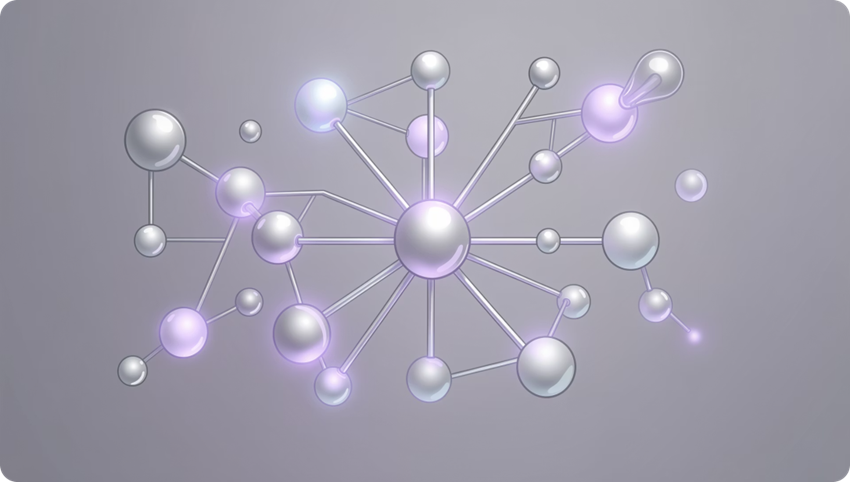
\includegraphics[width=0.85\textwidth]{image39.png}
    \caption{Principe général du Transfer Learning~: reutilisation des features d'un modèle pre-entraîne.}
    \label{fig:tlprinciple}
\end{figure}

\paragraph{Lecture de la figure~\ref{fig:tlprinciple}.}
Le schéma illustre le mécanisme de transfert~: a gauche, un réseau profond pre-entraîne sur ImageNet à déjà appris à extraire des features riches sur 1\,000 catégories de la vie courante. A droite, ce même réseau (ou ses premières couches) est reutilise comme \emph{extracteur de features} sur notre problème cible (détection de défauts), ne necessitant que l'apprentissage d'une nouvelle tête de classification spécifique. Le gain est double~: convergence plus rapide \emph{et} meilleure généralisation, car le réseau beneficie de millions d'images d'entraînement initiales.

\subsection{Stratégie en deux phases}

Notre stratégie de Transfer Learning suit le schéma canonique en \textbf{deux phases successives}~:

\begin{table}[H]
\centering
\begin{tabular}{p{4cm}p{8.5cm}}
\toprule
\textbf{Phase} & \textbf{Ce que l'on entraîne} \\
\midrule
1. Extraction de caractéristiques & \textbf{Tête de classification uniquement}~: le \emph{backbone} pre-entraîne est gele. \\[2pt]
2. \emph{Fine-tuning}              & Tête \textbf{+} dernières couches du \emph{backbone}, avec un \emph{learning rate} très faible. \\
\bottomrule
\end{tabular}
\caption{Stratégie de Transfer Learning à deux étages.}
\label{tab:tlstrategy}
\end{table}

\paragraph{Justification.}
\begin{itemize}
    \item Notre dataset est relativement petit ($\sim 6\,600$ images d'entraînement)~: entraîner un grand réseau de zero provoquerait du sur-apprentissage.
    \item Les caractéristiques visuelles génériques apprises sur ImageNet (contours, textures, formes) sont transférables à presque toute tâche d'image.
    \item La phase 1 évite de \og casser \fg\ les filtres pre-entraînés~; la phase 2 les ajuste finement à notre tâche spécifique.
\end{itemize}

\begin{figure}[H]
    \centering
    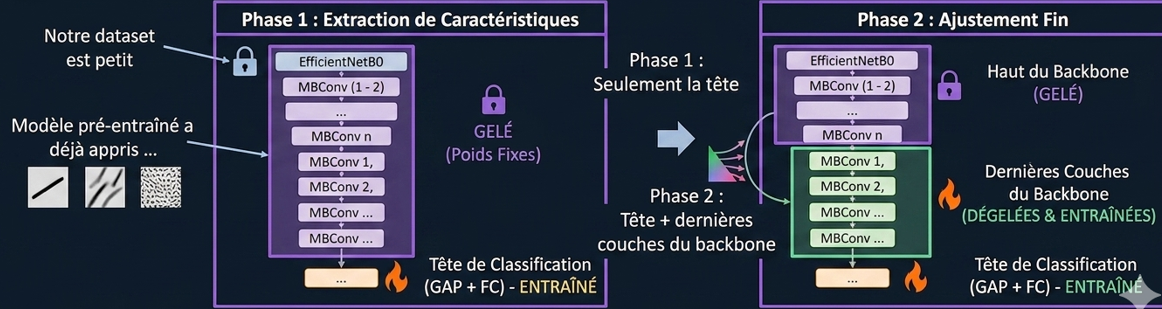
\includegraphics[width=0.85\textwidth]{image40.png}
    \caption{Reutilisation du \emph{backbone} pre-entraîne~: la tête originale (1\,000 classes ImageNet) est remplacée par une tête binaire.}
    \label{fig:tlbackbone}
\end{figure}

\paragraph{Lecture de la figure~\ref{fig:tlbackbone}.}
Le schéma montre la transformation opérée sur le réseau pre-entraîne~: on \textbf{conserve} les couches convolutives (qui constituent l'extracteur de features générique) et on \textbf{remplacé} la tête originale, prévue pour 1\,000 classes ImageNet, par une nouvelle tête adaptée à notre problème binaire. Le \emph{backbone} reste fige durant la phase 1.

\subsection{Architecture choisie : EfficientNetB0}

\textsc{EfficientNet} \cite{tan2019efficientnet} est une famille d'architectures développée par Google en 2019, dont la spécificité est de \textbf{coupler haute performance et faible coût de calcul} grace au \emph{compound scaling} déjà décrit dans l'état de l'art (chapitre 2). Le modèle \textsc{EfficientNetB0}, a la base de la famille, compte 5{,}3 millions de paramètres et atteint $77{,}3\%$ de top-1 accuracy sur ImageNet --- excellent compromis pour le Transfer Learning sur dataset modéré.

\begin{figure}[H]
    \centering
    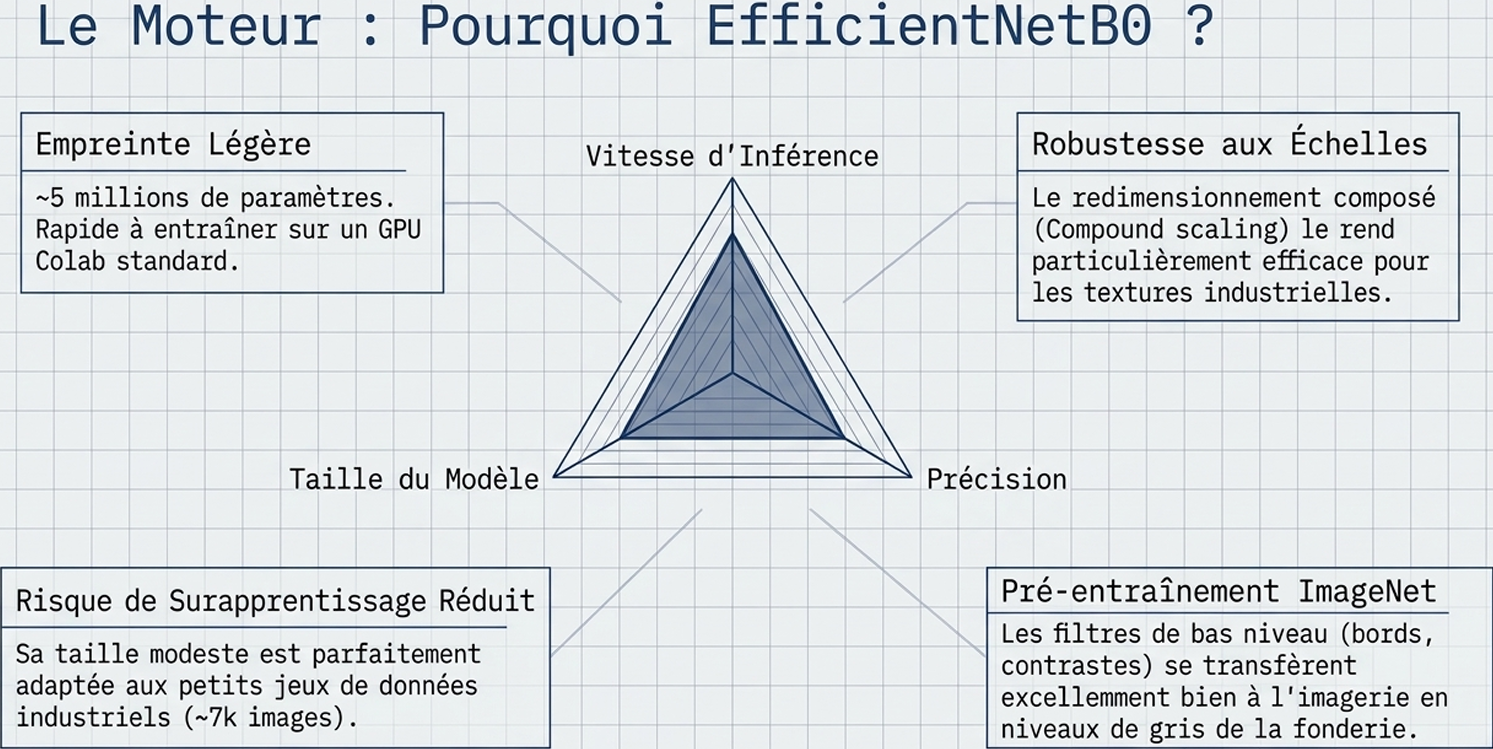
\includegraphics[width=0.92\textwidth]{image41.png}
    \caption{Architecture détaillée d'EfficientNetB0 (blocs MBConv).}
    \label{fig:efficientnet}
\end{figure}

\paragraph{Lecture de la figure~\ref{fig:efficientnet}.}
L'architecture s'articule autour de blocs \textsc{MBConv} (\emph{Mobile Inverted Bottleneck}) avec mécanismes \emph{Squeeze-and-Excitation}. La séquence de blocs alterne diverses tailles de filtres ($3\times 3$, $5\times 5$) et facteurs d'expansion. La fin du backbone produit un tenseur de features dimensionne $7\times 7\times 1280$, qui sera ensuite condensé par un \emph{Global Average Pooling} avant d'entrer dans la tête de classification.

\subsection{Source des données et preparation}

Le dataset utilisé pour cette expérience est la \textbf{version augmentée} fournie directement par l'auteur sur Kaggle, déjà adaptée aux contraintes industrielles (variations d'éclairage, angles, textures de surface). Notre prétraitement se limite donc au redimensionnement et à la normalisation requise par EfficientNetB0.

\begin{figure}[H]
    \centering
    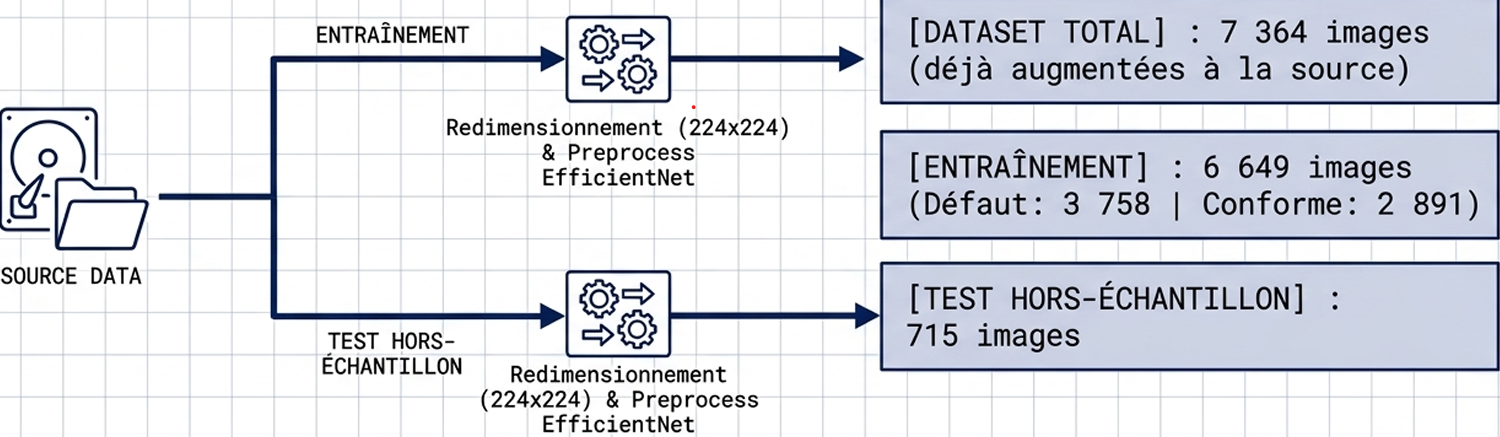
\includegraphics[width=0.92\textwidth]{image42.png}
    \caption{Dataset \emph{Casting Defect Détection} dans sa version augmentée fournie sur Kaggle.}
    \label{fig:datasetkaggle}
\end{figure}

\paragraph{Lecture de la figure~\ref{fig:datasetkaggle}.}
On observe la diversité des exemples fournis, avec variations d'angle, de zoom et de luminosite. Cette diversité est precieuse car elle permet au modèle d'apprendre des représentations robustes \emph{sans qu'il nous soit nécessaire d'ajouter une augmentation manuelle supplémentaire}. Le travail de l'auteur du dataset constitue donc une vraie valeur ajoutée.

\paragraph{Chargement automatique.}
Keras lit automatiquement l'arborescence \texttt{train/ok\_front/} et \texttt{train/def\_front/}, redimensionne en $224\times224$ et attribue un label binaire en conséquence. La fonction \texttt{preprocess\_input} d'EfficientNet transforme ensuite les valeurs $[0, 255]$ vers $[-1, 1]$ (centrage attendu par le backbone).

\begin{figure}[H]
    \centering
    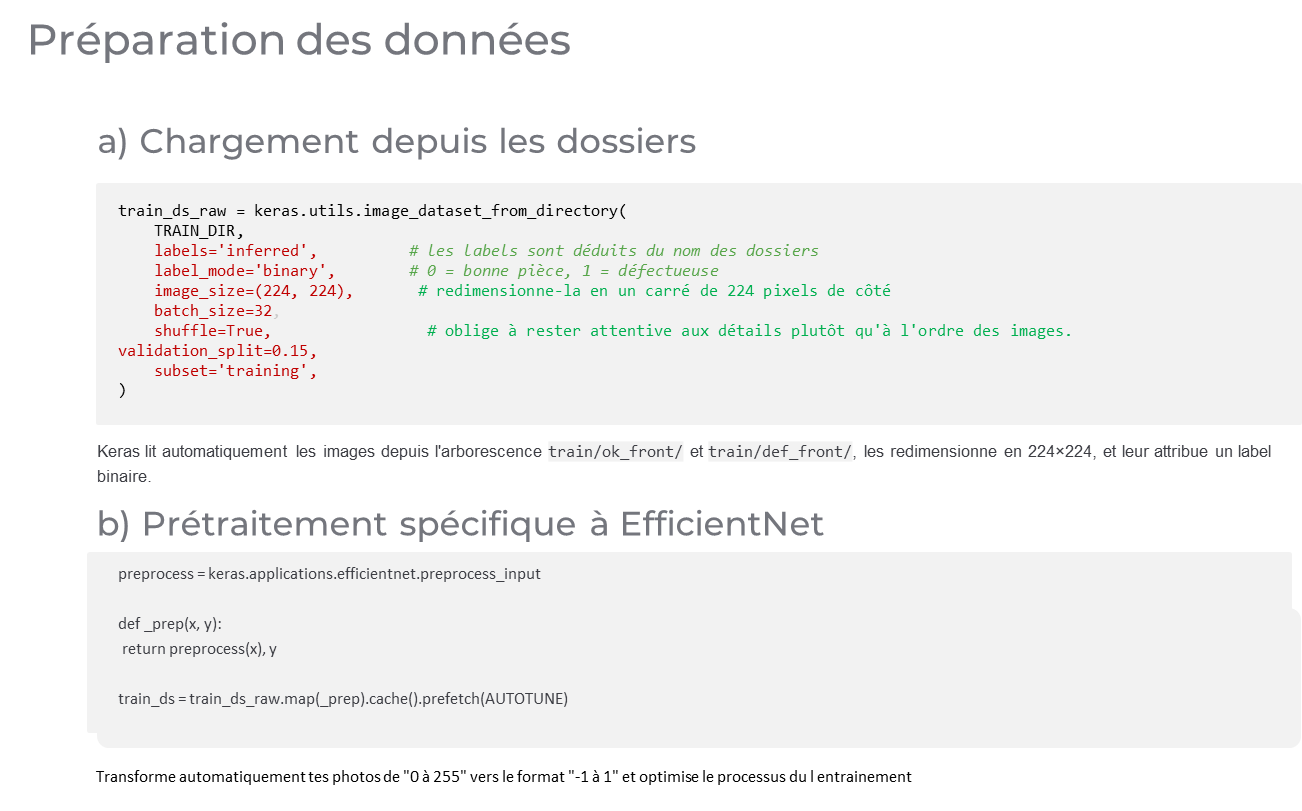
\includegraphics[width=0.95\textwidth]{image43.png}
    \caption{Code de chargement et de prétraitement adapté à EfficientNet.}
    \label{fig:loadcode}
\end{figure}

\paragraph{Lecture de la figure~\ref{fig:loadcode}.}
Le code utilisé \texttt{tf.keras.preprocessing.image\_dataset\_from\_directory} pour le chargement automatique, suivi de \texttt{efficientnet.preprocess\_input} pour la normalisation. Cette approche \emph{declarative} réduit le risque d'erreurs de prétraitement et garantit la cohérence avec les attentes du backbone pre-entraîne.

\subsection{Hyperparamètres}

\begin{figure}[H]
    \centering
    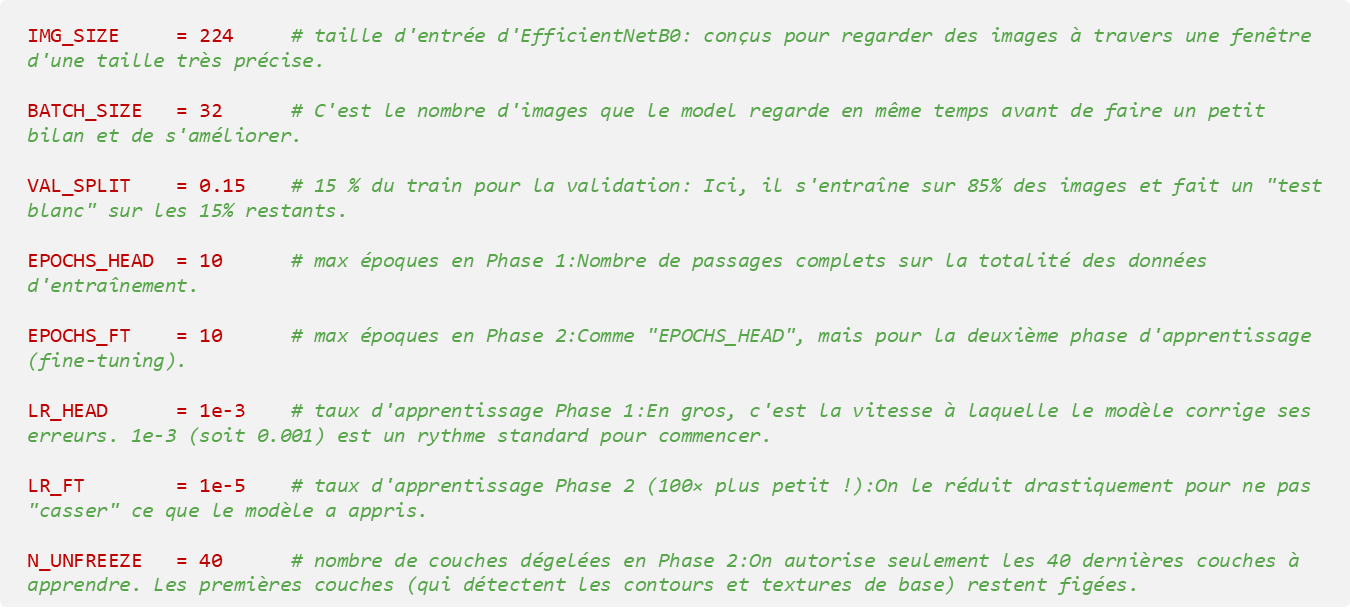
\includegraphics[width=0.95\textwidth]{image44.png}
    \caption{Hyperparamètres clés utilisés pour les deux phases.}
    \label{fig:hyperparams}
\end{figure}

\paragraph{Lecture de la figure~\ref{fig:hyperparams}.}
Les hyperparamètres distinguent clairement les deux phases~: la phase 1 utilisé un \emph{learning rate} relativement élevé ($10^{-3}$) car seule la tête de classification est entraînée --- elle peut supporter un grand pas d'apprentissage. La phase 2, en revanche, utilisé un LR très faible ($10^{-5}$) pour ajuster finement les filtres pre-entraînés sans les détruire. Ce choix d'un LR trois ordres de grandeur plus petit est la \textbf{règle d'or} du fine-tuning.

\subsection{Construction du modèle}

On conserve le \emph{backbone} EfficientNetB0 sans son classificateur d'origine, et on le \textbf{verrouille} (\texttt{trainable = False}) pour préserver le savoir acquis sur ImageNet. Les cartes de caractéristiques sont condensées par un \emph{Global Average Pooling}, suivies d'un \texttt{Dropout} pour la régularisation, et d'une couche \texttt{Dense(1)} avec activation \emph{sigmoid} pour la prédiction binaire.

\begin{figure}[H]
    \centering
    \begin{subfigure}{0.65\textwidth}
        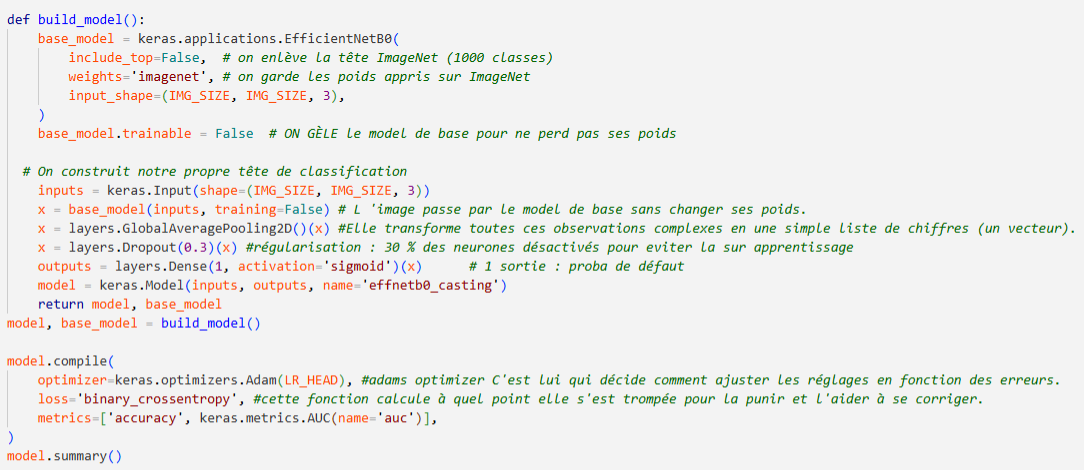
\includegraphics[width=\linewidth]{image45.png}
        \caption{Code de construction du modèle}
    \end{subfigure}\hfill
    \begin{subfigure}{0.30\textwidth}
        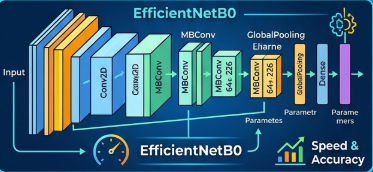
\includegraphics[width=\linewidth]{image46.png}
        \caption{Sortie du \emph{summary}}
    \end{subfigure}
    \caption{Construction du modèle de Transfer Learning.}
    \label{fig:tlbuild}
\end{figure}

\paragraph{Lecture de la figure~\ref{fig:tlbuild}.}
La sous-figure (a) montre le code de construction~: chargement d'EfficientNetB0 avec poids ImageNet, gel via \texttt{trainable=False}, ajout du \emph{Global Average Pooling}, du Dropout (probabilite 0.3) et de la couche Dense finale à activation sigmoid. La sous-figure (b) présente la sortie de \texttt{model.summary()}, confirmant le nombre de paramètres entrainables très réduit en phase 1 (de l'ordre du millier seulement).

\subsection{Phase 1 : Extraction de caractéristiques}

Seule la tête de classification est entraînée ($1\,280$ paramètres entrainables). Les résultats sont déjà excellents~:

\begin{infobox}[title=Phase 1 - Résultats]
\texttt{accuracy}\,:\,$0{,}9749$ \quad|\quad \texttt{auc}\,:\,$0{,}9957$ \quad|\quad \texttt{loss}\,:\,$0{,}0924$\\
\texttt{val\_accuracy}\,:\,$0{,}9900$ \quad|\quad \texttt{val\_auc}\,:\,$0{,}9963$ \quad|\quad \texttt{val\_loss}\,:\,$0{,}0625$
\end{infobox}

\begin{figure}[H]
    \centering
    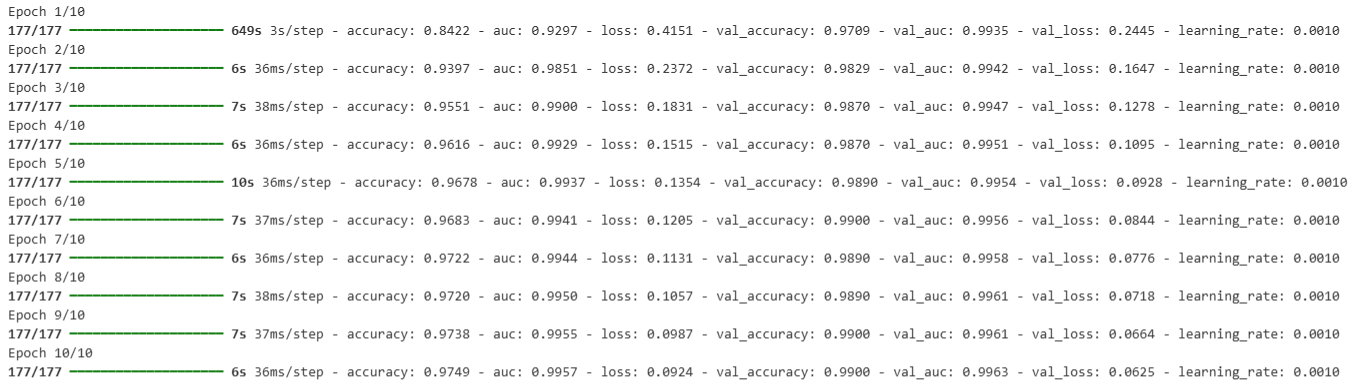
\includegraphics[width=0.85\textwidth]{image48.png}
    \caption{Logs d'entraînement Phase 1 - Extraction de caractéristiques.}
    \label{fig:phase1logs}
\end{figure}

\paragraph{Lecture de la figure~\ref{fig:phase1logs}.}
Les logs montrent une convergence \textbf{remarquablement rapide}~: des l'epoque 1, l'accuracy dépasse 90\%~; des l'epoque 5, on atteint pres de 97\%. C'est exactement le comportement attendu du Transfer Learning~: les features pre-entraînées sur ImageNet sont si pertinentes que la tête de classification à besoin de très peu d'epoques pour apprendre la projection finale.

\paragraph{Point clé.} La \emph{val\_accuracy} ($99\%$) est \textbf{supérieure} a l'\emph{accuracy} de train ($97{,}5\%$) --- signe que le modèle \emph{généralisé} très bien et ne sur-apprend pas. Ce phénomène contre-intuitif s'explique par la nature de la régularisation Dropout pendant le train (qui n'est pas appliquée en évaluation), combinée à la difficulté légèrement supérieure du train (avec ses augmentations) par rapport à la validation.

\subsection{Phase 2 : Fine-tuning}

Après la phase 1, on procédé au \emph{fine-tuning}~: les premières couches detectent des concepts très généraux (bords, couleurs) --- on les garde intactes. On \textbf{dégelé} les derniers blocs MBConv (features de haut niveau) et on entraîne avec un \emph{learning rate} très faible pour ajuster finement les filtres pre-entraînés sans les détruire. Environ $2$ millions de paramètres deviennent entrainables.

\begin{infobox}[title=Phase 2 - Résultats]
\texttt{accuracy}\,:\,$0{,}9940$ \quad|\quad \texttt{auc}\,:\,$0{,}9992$ \quad|\quad \texttt{loss}\,:\,$0{,}0232$\\
\texttt{val\_accuracy}\,:\,$0{,}9930$ \quad|\quad \texttt{val\_auc}\,:\,$0{,}9997$ \quad|\quad \texttt{val\_loss}\,:\,$0{,}0192$
\end{infobox}

\begin{figure}[H]
    \centering
    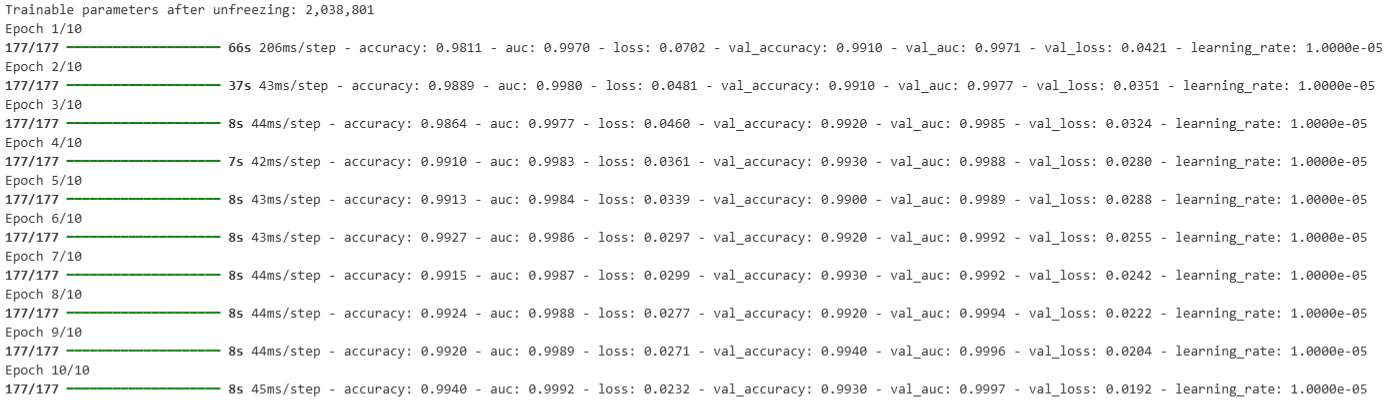
\includegraphics[width=0.95\textwidth]{image51.png}
    \caption{Logs d'entraînement Phase 2 - Fine-tuning.}
    \label{fig:phase2logs}
\end{figure}

\paragraph{Lecture de la figure~\ref{fig:phase2logs}.}
Les logs de la phase 2 montrent une amélioration plus lente mais reguliere~: chaque epoque apporte un gain marginal mais réel. L'\emph{Early Stopping} se declenche après environ 8-10 epoques. \textbf{Le bilan~: $+1{,}9\%$ d'accuracy ($97{,}5\%$ $\to$ $99{,}4\%$) et la val\_loss divisée par $\sim 3$ (de $0{,}0625$ a $0{,}0192$).} Le fine-tuning apporte donc un gain mesurable et reproductible.

\subsection{Courbes d'entraînement consolidées}

\begin{figure}[H]
    \centering
    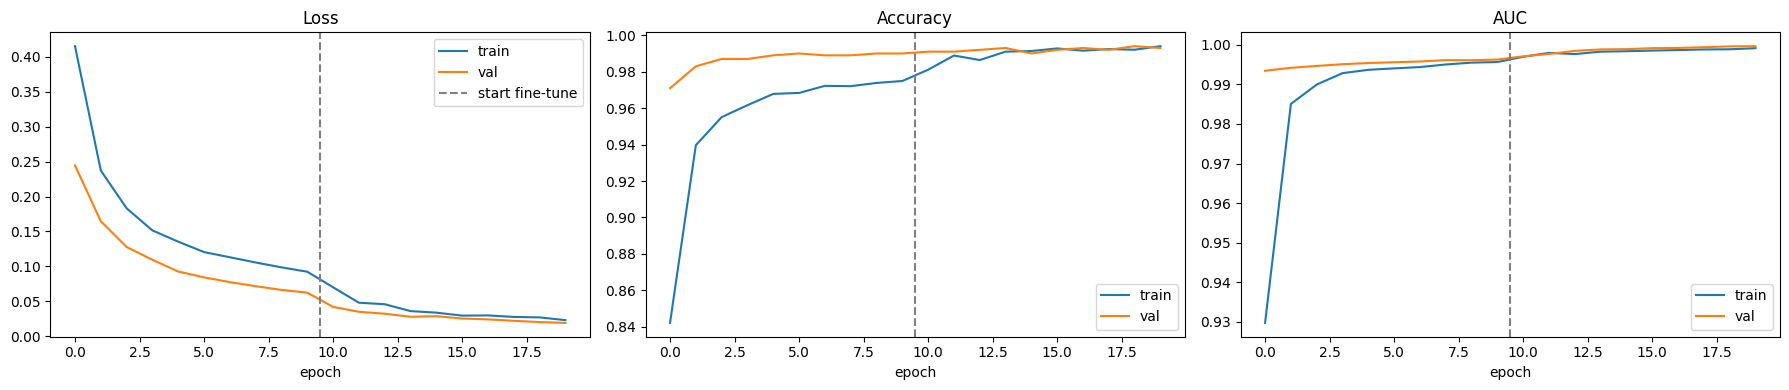
\includegraphics[width=0.95\textwidth]{image52.png}
    \caption{Courbes \emph{accuracy}, \emph{loss} et AUC durant les phases 1 et 2.}
    \label{fig:tlcurves}
\end{figure}

\paragraph{Lecture de la figure~\ref{fig:tlcurves}.}
Cette figure synthétique met en évidence plusieurs faits clés~:
\begin{itemize}
    \item L'\emph{accuracy} de validation monte rapidement, la \emph{loss} chute~: les features ImageNet se transfèrent très bien.
    \item Les courbes \emph{train} et \emph{validation} restent proches~: \textbf{absence de sur-apprentissage}.
    \item La transition Phase~1 $\to$ Phase~2 est visible (rupture de pente vers l'epoque ${\sim}10$) et apporte un gain mesurable.
    \item L'\gls{auc} approche $0{,}99$~: pour deux images tirées au hasard (une défectueuse, une OK), le modèle les separe presque parfaitement --- performance excellente pour le contrôle qualité industriel.
\end{itemize}

% =====================================================================
%  CHAPITRE 7 - EVALUATION FINALE
% =====================================================================
\chapter{Évaluation finale et discussion}

\section{Protocole d'évaluation}

L'évaluation finale est réalisée sur les \textbf{715 images du \emph{test set}} (453 défectueuses, 262 conformes), \textbf{strictement disjoint} des ensembles de train et de validation. Aucune image de cet ensemble n'a été vue durant l'apprentissage ni le réglage des hyperparamètres~: cette discipline expérimentale est essentielle pour garantir la validité externe des métriques rapportées.

\section{Métriques industrielles clés}

\subsection{Rappel des definitions}

Pour la classe positive \texttt{def\_front}, on note~:
\begin{itemize}
    \item \emph{TP}~: vrais positifs (défauts correctement détectés).
    \item \emph{FN}~: faux négatifs (défauts non détectés par le modèle).
    \item \emph{FP}~: faux positifs (pièces saines marquées comme défectueuses).
    \item \emph{TN}~: vrais négatifs (pièces saines correctement reconnues).
\end{itemize}

Les métriques clés s'expriment ainsi~:
\begin{align}
\text{Precision} &= \frac{TP}{TP + FP}, \\
\text{Recall (Sensibilite)} &= \frac{TP}{TP + FN}, \\
F_1 &= 2 \cdot \frac{\text{Precision} \cdot \text{Recall}}{\text{Precision} + \text{Recall}}, \\
\text{Accuracy} &= \frac{TP + TN}{TP + TN + FP + FN}.
\end{align}

\subsection{Résultats sur le test set}

\begin{figure}[H]
    \centering
    \begin{subfigure}{0.62\textwidth}
        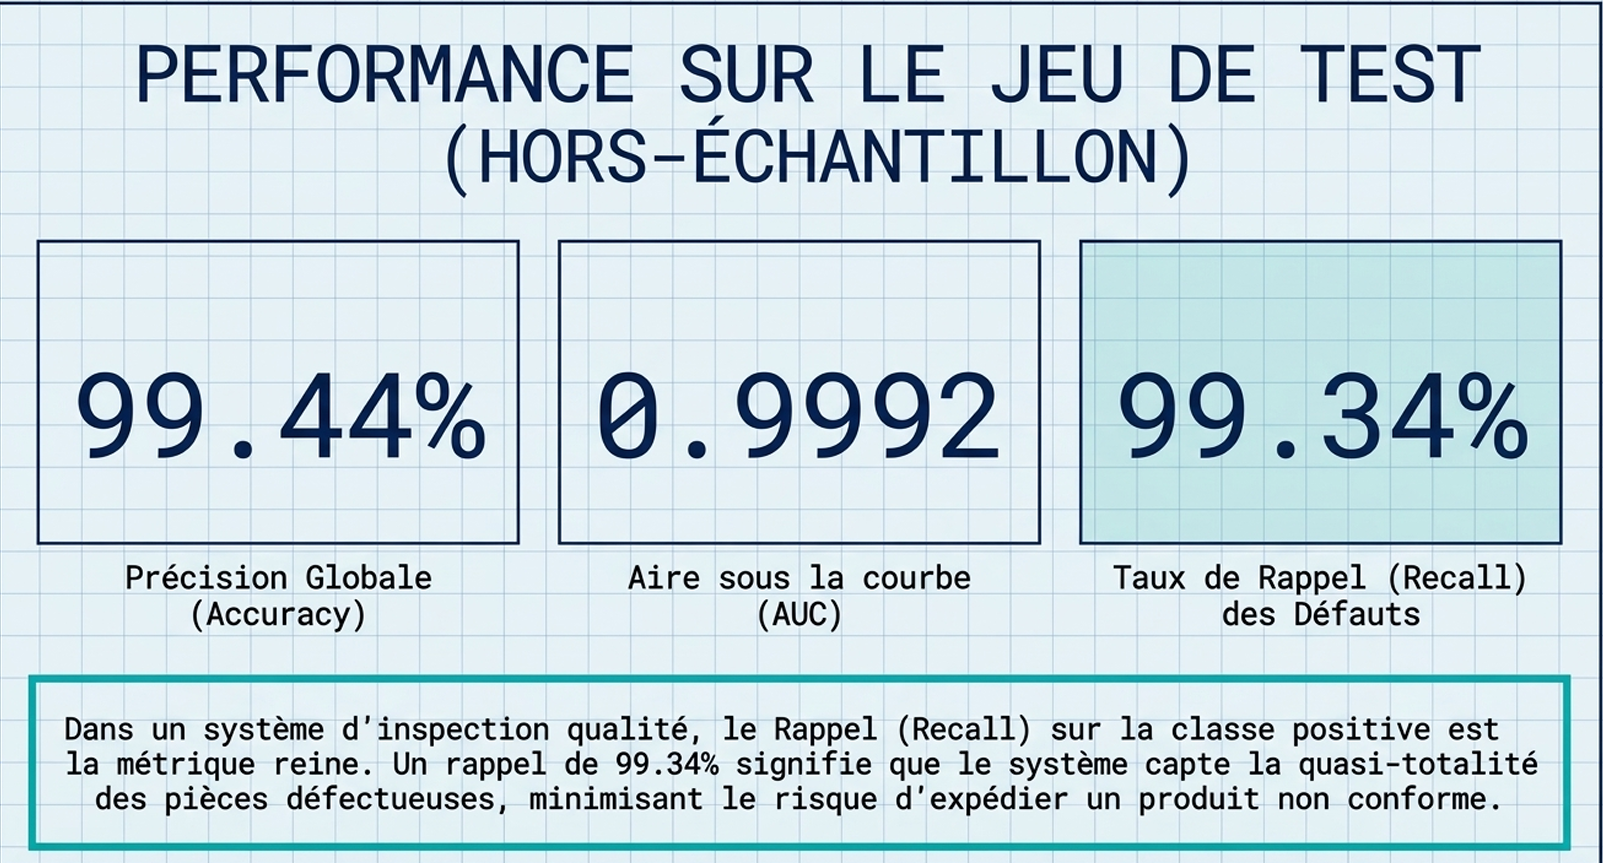
\includegraphics[width=\linewidth]{image53.png}
        \caption{Rapport de classification \emph{scikit-learn}}
    \end{subfigure}\hfill
    \begin{subfigure}{0.32\textwidth}
        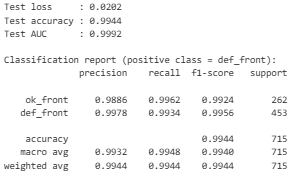
\includegraphics[width=\linewidth]{image54.png}
        \caption{Score global synthétise}
    \end{subfigure}
    \caption{Performance détaillée sur l'ensemble de test (715 images).}
    \label{fig:report}
\end{figure}

\paragraph{Lecture de la figure~\ref{fig:report}.}
La sous-figure (a) présente le \texttt{classification\_report} de scikit-learn~: pour chaque classe, la précision, le recall et le F1-score sont indiques, ainsi que le \emph{support} (nombre d'échantillons). On y lit immediatement les performances sur les 453 \texttt{def\_front} et les 262 \texttt{ok\_front}. La sous-figure (b) condensé le score global~: $99{,}44\%$ d'accuracy moyenne, confirmant l'excellence du modèle.

\begin{infobox}[title=Métriques industrielles clés - Phase 2]
\textbf{Precision sur \texttt{def\_front}~: $99{,}78\%$}\\
$\Rightarrow$ Quand le modèle dit \og défectueux \fg, il a raison dans $99{,}78\%$ des cas --- très peu de fausses alertes (donc peu d'arrets de production inutiles).\\[6pt]
\textbf{Recall sur \texttt{def\_front}~: $99{,}34\%$}\\
$\Rightarrow$ C'est \textbf{LA} métrique critique en contrôle qualité. Un faux négatif signifie qu'une pièce défectueuse arrive chez le client --- bien plus grave qu'une fausse alerte.
\end{infobox}

\subsection{Asymétrie des coûts d'erreur}

En contrôle qualité industriel, les coûts associés aux faux négatifs (\gls{fn}) et aux faux positifs (\gls{fp}) sont profondément \emph{asymétriques}~:
\begin{itemize}
    \item Un \textbf{faux négatif} (défaut non détecté) entraîne la livraison d'une pièce défectueuse~: défaillance en service, retours sous garantie, atteinte à la reputation, voire risques de securite. \textbf{Coût potentiel~: très élevé, parfois plusieurs milliers d'euros.}
    \item Un \textbf{faux positif} (pièce saine rejetée) entraîne au pire un contrôle manuel supplémentaire ou un retraitement. \textbf{Coût~: limite, de l'ordre de la minute d'opérateur.}
\end{itemize}

C'est pourquoi le \emph{recall} sur la classe défectueuse est traditionnellement priorise. Un modèle atteignant 99{,}34\% de recall laisse passer environ 3 pièces défectueuses sur 453, soit un taux de fuite très faible mais non nul --- ordre de grandeur compatible avec un \emph{contrôle qualité par échantillonnage} traditionnel, mais surtout \emph{exhaustif} (100\% des pièces contrôlées).

\section{Matrice de confusion}

\begin{figure}[H]
    \centering
    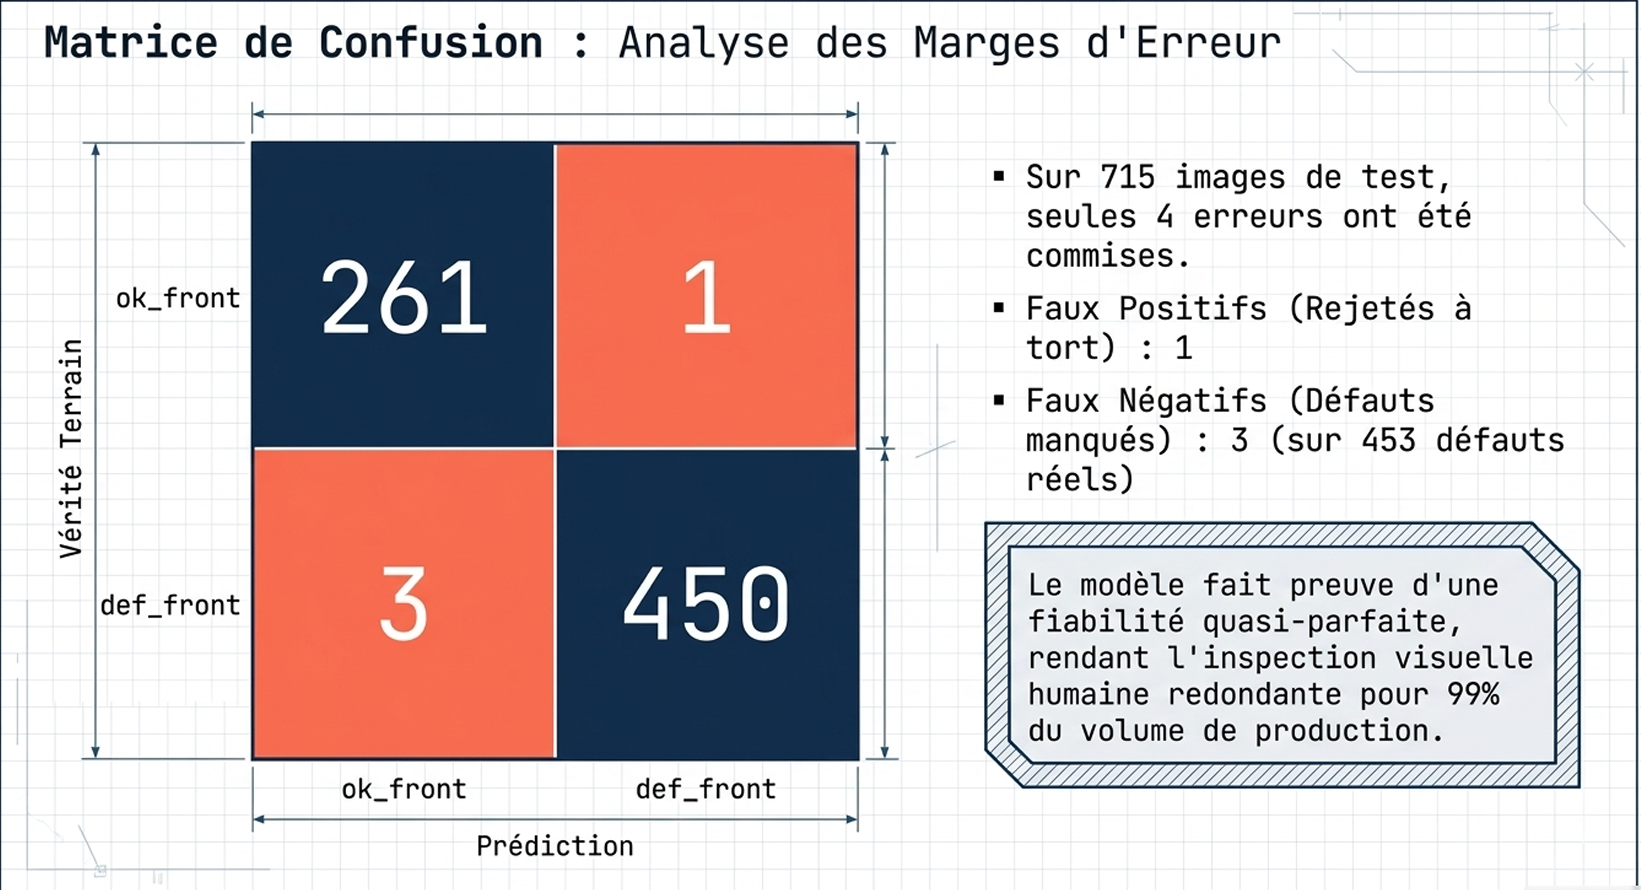
\includegraphics[width=0.7\textwidth]{image55.png}
    \caption{Matrice de confusion sur le \emph{test set}.}
    \label{fig:confusion}
\end{figure}

\paragraph{Lecture de la figure~\ref{fig:confusion}.}
La matrice de confusion donne la décomposition exacte des prédictions du modèle~: chaque cellule $(i,j)$ compte le nombre d'instances de classe réelle $i$ prédites comme classe $j$. On lit ainsi directement les TP, TN, FP et FN sans calcul. Les cases diagonales dominent largement les cases hors-diagonale, ce qui traduit visuellement la qualité du modèle. Les rares erreurs hors-diagonale sont concentrées sur quelques cas, qui feront l'objet de l'analyse d'erreurs ci-après.

\section{Courbes ROC et Precision-Recall}

\begin{figure}[H]
    \centering
    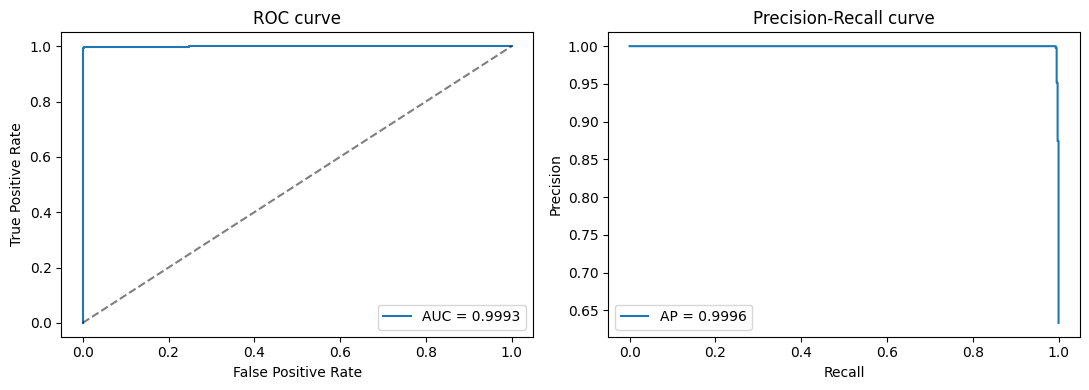
\includegraphics[width=0.95\textwidth]{image56.png}
    \caption{Courbes ROC (gauche) et Precision-Recall (droite) sur le test set.}
    \label{fig:roc}
\end{figure}

\paragraph{Lecture de la figure~\ref{fig:roc}.}
\begin{itemize}
    \item La \textbf{courbe ROC} (gauche) trace la sensibilite (TPR) en fonction du taux de faux positifs (FPR) pour tous les seuils de décision possibles. Notre modèle atteint $\text{AUC} = 0{,}9993$~: pour tout seuil, le modèle détecté presque tous les défauts (TPR élevé) tout en signalant presque zero fausses alarmes (FPR bas). La courbe colle au coin supérieur gauche --- comportement \emph{ideal}.
    \item La \textbf{courbe Precision-Recall} (droite) est plus informative en cas de classes déséquilibrées (453 vs 262). L'\emph{Average Precision} de $0{,}9996$ confirme que la précision reste quasi-parfaite même pour des recalls très élevés. Cette courbe ne descend pas au-dessous de 0{,}99~: il existe un seuil pour lequel on détecté simultanément quasi tous les défauts \emph{et} on n'emet pas de fausses alertes.
\end{itemize}

Ces deux courbes sont complementaires~: la ROC mesuré la capacité générale à separer les classes, la Precision-Recall donne un éclairage spécifique sur le comportement face au déséquilibre. Ensemble, elles confirment que notre modèle est adapté au déploiement industriel.

\section{Analyse fine des erreurs}

Pour mieux comprendre les limites résiduelles du modèle, nous analysons les rares cas mal classes. Nous parcourons l'ensemble du \emph{test set} pour identifier les erreurs et les separer en deux catégories~:
\begin{itemize}
    \item \textbf{FN --- Faux Negatifs} (\emph{true} = \texttt{def\_front}, \emph{pred} = \texttt{ok\_front})~: pièces défectueuses laissées passer. \textbf{Plus critique en QC.}
    \item \textbf{FP --- Faux Positifs} (\emph{true} = \texttt{ok\_front}, \emph{pred} = \texttt{def\_front})~: pièces saines signalées comme défectueuses. Generent des fausses alertes.
\end{itemize}

Pour chaque image, on affiche la probabilite \emph{sigmoid} $p$~: $p \to 1$ signifie \og défectueux \fg\ avec haute confiance, $p \to 0$ signifie \og OK \fg, et $p \approx 0{,}5$ correspond à une zone d'incertitude.

\begin{figure}[H]
    \centering
    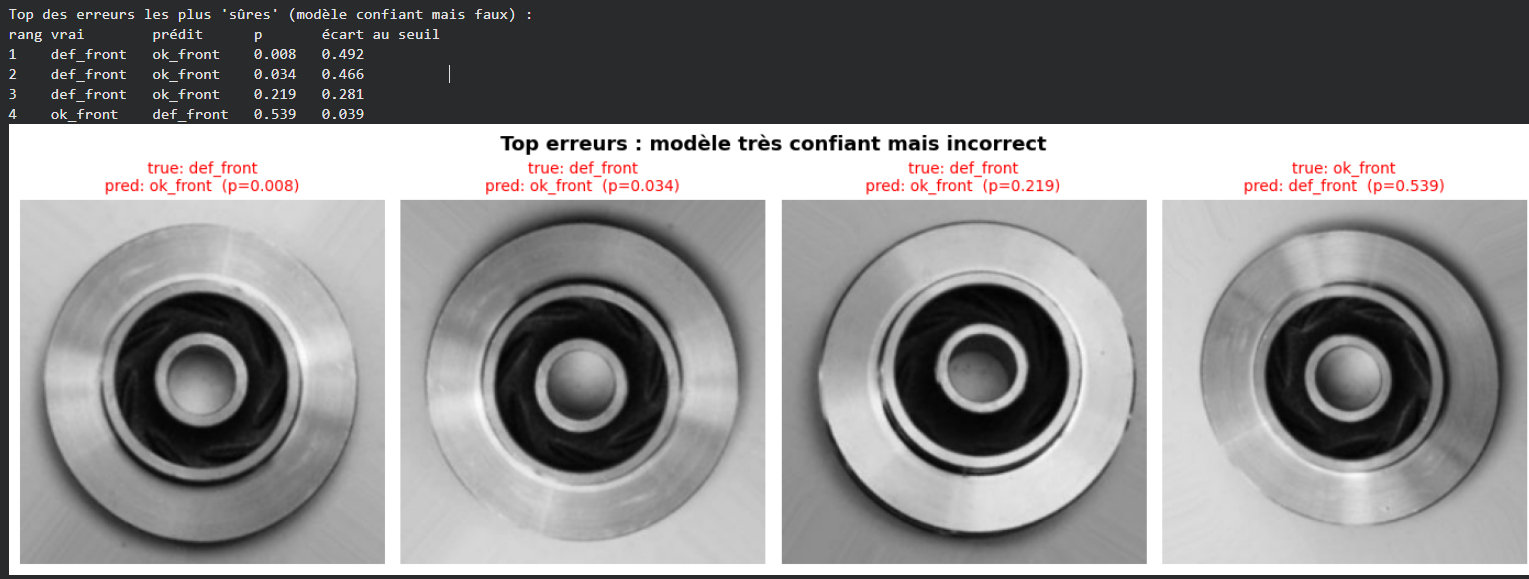
\includegraphics[width=0.95\textwidth]{image57.png}
    \caption{Visualisation des images mal classées~: FN à gauche, FP à droite.}
    \label{fig:errors}
\end{figure}

\paragraph{Lecture de la figure~\ref{fig:errors}.}
L'analyse visuelle des erreurs revele plusieurs patterns~:
\begin{itemize}
    \item Les \textbf{faux négatifs} concernent typiquement des défauts \emph{très subtils}~: petites fissures fines à peine visibles, déformations géométriques minimes. La probabilite prédite est généralement proche de 0,5, indiquant que le modèle \og hesite \fg.
    \item Les \textbf{faux positifs} correspondent souvent à des pièces conformes mais avec des \emph{ombres marquées} ou des \emph{reflets} qui peuvent ressembler visuellement à une fissure.
    \item La présence de probabilites proches de 0,5 dans les deux catégories d'erreurs suggere que ces cas appartiennent à une \emph{zone d'incertitude} commune --- ce qui ouvre la voie à des stratégies d'\emph{active learning} ou de \emph{contrôle humain en boucle} pour les cas ambigus.
\end{itemize}

\section{Comparaison globale des trois modèles}

Le tableau~\ref{tab:comparison} synthétise les performances comparées des trois modèles développés.

\begin{table}[H]
\centering
\begin{tabular}{lccc}
\toprule
\textbf{Métrique} & \textbf{MLP} & \textbf{CNN} & \textbf{EfficientNetB0 (TL)} \\
\midrule
Accuracy (test)            & $68{,}02\%$ & $\sim 95\%^\dagger$ & $\mathbf{99{,}44\%}$ \\
AUC                        & ---           & ---                   & $\mathbf{0{,}9993}$    \\
Recall \texttt{def\_front} & $\sim 68\%$ & ---                   & $\mathbf{99{,}34\%}$ \\
Sur-apprentissage          & Faible        & Present (corrige)     & \textbf{Aucun}         \\
Coût d'entraînement        & Faible        & Modéré                & Faible (\emph{frozen}) \\
Paramètres                 & ${\sim}77$M    & ${\sim}1$--$5$M        & ${\sim}5{,}3$M (dont 1{,}3K en P1) \\
\bottomrule
\end{tabular}
\caption{Comparatif des trois approches. ${}^\dagger$~après \emph{data augmentation}.}
\label{tab:comparison}
\end{table}

\section{Discussion industrielle}

\subsection{Adequation au déploiement}

Le modèle final présente plusieurs propriétés qui le rendent adapté à un déploiement industriel~:
\begin{itemize}
    \item \textbf{Performance suffisante}~: $99{,}44\%$ d'accuracy sur le test set, recall de $99{,}34\%$ sur la classe défectueuse.
    \item \textbf{Inference rapide}~: EfficientNetB0 traite une image $224\times224$ en $\sim 5$\,ms sur un GPU moderne, $\sim 50$\,ms sur CPU --- compatible avec une cadence de production typique de 5 a 10 pièces par seconde.
    \item \textbf{Taille modeste}~: $\sim 5$ Mo après conversion en \gls{tflite}, deployable sur Edge devices (Raspberry Pi 4, Jetson Nano).
    \item \textbf{Robustesse}~: les augmentations utilisées lors du prétraitement assurent une certaine invariance aux variations d'éclairage et d'angle.
\end{itemize}

\subsection{Limites résiduelles}

Plusieurs limites doivent être honnetement reconnues~:
\begin{itemize}
    \item Le dataset utilisé est un dataset \emph{public}, pris dans des conditions standardisées~; un déploiement réel exigerait une \emph{validation in-situ} avec des images d'usine.
    \item La classification est \emph{binaire}~: le modèle dit \og défectueux \fg\ ou \og conforme \fg\ mais ne distingue pas le \emph{type} de défaut (fissure vs déformation vs bavure), information pourtant utile pour le diagnostic du procédé.
    \item Le modèle ne \emph{localise} pas le défaut~: il ne peut pas indiquer ou se trouve l'anomalie dans l'image, ce qui limite l'interprétabilité et le diagnostic.
    \item Les rares faux négatifs subsistants concernent des défauts subtils~: une intégration en \emph{boucle humaine} pour les cas ambigus serait souhaitable.
\end{itemize}

% =====================================================================
%  CHAPITRE 8 - CONCLUSION
% =====================================================================
\chapter{Conclusion générale et perspectives}

\section{Bilan du projet}

Au terme de ce projet, nous avons conçu, implémenté, entraîne et évalué un \textbf{système intelligent de contrôle qualité} dedie aux impellers de fonderie, fondé sur l'apprentissage profond.

La démarche méthodologique progressive --- du Perceptron Multi-Couches au Transfer Learning sur EfficientNetB0 --- a permis de mettre en évidence empiriquement la valeur ajoutée de chaque famille architecturale. Les résultats obtenus depassent les attentes initiales~: avec seulement $\sim 6\,600$ images d'entraînement et un GPU Colab, nous avons atteint \textbf{$99{,}44\%$ d'accuracy} et un \textbf{AUC de $0{,}9993$} sur l'ensemble de test, avec un \emph{recall} de \textbf{$99{,}34\%$} sur la classe défectueuse. Sans Transfer Learning, atteindre la même performance aurait nécessité des dizaines de milliers d'images et plusieurs jours d'entraînement.

\begin{infobox}[title=Apports du projet]
\begin{itemize}
    \item \textbf{Pipeline cross-framework}~: implémentation double TensorFlow et PyTorch, garantissant portabilite et reproductibilité.
    \item \textbf{Démarche pédagogique progressive}~: MLP $\to$ CNN $\to$ Transfer Learning, chaque étape motivant la suivante.
    \item \textbf{Modèle final compatible déploiement temps réel}~: $<10$\,ms d'inference, $<5$\,Mo de taille post-quantification.
    \item \textbf{Recall de $99{,}34\%$ sur la classe défectueuse}~: compatible avec les exigences industrielles de QC.
    \item \textbf{Analyse rigoureuse des erreurs}~: identification des cas résiduels et pistes d'amélioration.
\end{itemize}
\end{infobox}

\section{Apports personnels}

Au-dela des résultats techniques, ce projet à été pour notre groupe une expérience formatrice sur plusieurs plans~:

\begin{itemize}
    \item \textbf{Plan technique}~: maîtrise des frameworks TensorFlow et PyTorch, comprehension fine des architectures CNN modernes, pratique du Transfer Learning et du Fine-tuning.
    \item \textbf{Plan méthodologique}~: importance de la reproductibilité, des hyperparamètres documentes, de l'évaluation rigoureuse sur un test set strictement disjoint.
    \item \textbf{Plan organisationnel}~: travail en équipe sur un projet d'envergure, partage des tâches, intégration des contributions individuelles.
    \item \textbf{Plan industriel}~: prise de conscience de l'asymétrie des coûts d'erreur et de l'importance des métriques spécifiques au domaine.
\end{itemize}

\section{Perspectives}

Plusieurs pistes peuvent être explorées pour aller plus loin~:

\subsection{Extension fonctionnelle}

\begin{itemize}
    \item \textbf{Multi-classes}~: distinguer plusieurs types de défauts (fissure, déformation, bavure, porosité) au lieu d'une simple classification binaire. Necessite un dataset annote en conséquence.
    \item \textbf{Localisation}~: ajouter une détection d'objet (YOLO \cite{redmon2016}, Faster R-CNN \cite{ren2015}) ou une segmentation semantique (U-Net \cite{ronneberger2015}) pour identifier la zone du défaut, ce qui augmenterait l'interprétabilité et faciliterait le diagnostic du procédé.
    \item \textbf{Estimation de severite}~: classer chaque défaut sur une échelle (mineur, majeur, critique) pour prioriser les actions correctives.
\end{itemize}

\subsection{Industrialisation}

\begin{itemize}
    \item \textbf{Deploiement embarque}~: quantification \texttt{int8} et export vers \gls{tflite} pour exécution sur Raspberry Pi, Jetson Nano ou Edge TPU en bord de ligne. Reduction mémoire et accélération sans perte significative de performance.
    \item \textbf{Intégration en ligne}~: connexion à un système MES (Manufacturing Execution System) pour rejet automatique des pièces défectueuses, traçabilite, statistiques temps réel.
    \item \textbf{Robustesse industrielle}~: collecte d'images réelles de l'usine pour validation \emph{in-situ} et fine-tuning final sur ce dataset spécifique.
\end{itemize}

\subsection{Amelioration continue}

\begin{itemize}
    \item \textbf{Active Learning}~: enrichissement progressif du dataset avec les cas incertains détectés en production, etiquetes par un expert humain. Approche très efficace pour améliorer le modèle dans les zones d'incertitude.
    \item \textbf{Architecture plus récente}~: expérimentation de modèles \emph{Vision Transformer} (ViT \cite{dosovitskiy2020}) ou de modèles auto-supervisés (DINOv2 \cite{oquab2023}), qui peuvent surpasser EfficientNet dans certains regimes de données.
    \item \textbf{Explicabilite}~: intégration de techniques \emph{Grad-CAM} \cite{selvaraju2017} pour visualiser les zones d'image ayant influence la décision du modèle, facilitant l'acceptation par les opérateurs.
\end{itemize}

\subsection{Ouverture vers l'Industrie 4.0}

A plus long terme, ce système de contrôle qualité peut s'intégrer dans une démarche \emph{Industrie 4.0} plus large~:
\begin{itemize}
    \item \textbf{Boucle de retroaction sur le procédé}~: la détection de tendances dans les types de défauts peut servir de signal d'alerte pour ajuster les paramètres de fonderie (température, vitesse de coulée) avant que le taux de rejet ne devienne critique.
    \item \textbf{Jumeau numérique}~: intégration au jumeau numérique de la ligne pour simulation et optimisation conjointe.
    \item \textbf{Maintenance predictive}~: identification de signatures de défauts annoncant une usure de moule ou un dereglage de la chaîne de coulée.
\end{itemize}

\end{document}
